\documentclass[12pt,fleqn]{article}\usepackage{../common}
\begin{document}
Ekler (Appendix) 

Cok Boyutlu Gaussian'i Parcalamak (Partitioning)

Diyelim ki Normal bir vektor $X$'i $X = (X_1,X_2)$ olarak parcaladik. Bunu
Gaussian'a etkileri ne olur? Ayni sekilde $\mu = (\mu_1,\mu_2)$ olarak
parcalayabiliriz. $\Sigma$ ise

\[ \Sigma = 
\left[\begin{array}{rr}
\Sigma_{11} & \Sigma_{12}\\
\Sigma_{21} & \Sigma_{22}
\end{array}\right]
 \]

olarak parcalanabilir. $a,b$'nin parcalarinin boyutlari $p,q$ olsun, $n =
p+q$.

Simdi birlesik Gaussian'i 

\[ f(x;\mu,\Sigma) = 
\frac{ 1}{(2\pi)^{(p+q)/2} \det(\Sigma)^{1/2}} 
\exp 
\bigg\{ 
-\frac{ 1}{2}
\left[\begin{array}{r}
x_1 - \mu_1\\
x_2 - \mu_2
\end{array}\right]^T
\left[\begin{array}{rr}
\Sigma_{11} & \Sigma_{12}\\
\Sigma_{21} & \Sigma_{22}
\end{array}\right]^{-1}
\left[\begin{array}{r}
x_1 - \mu_1\\
x_2 - \mu_2
\end{array}\right]
\bigg\}
 \]

Birlesik yogunlugu parcalar uzerinden belirtirsek, bu yogunlugu $X_2$ icin
bilesen yogunluga ve $X_1$ icin bir kosullu yogunluga ayirabiliriz. Yani 

\[ f(x_1,x_2) = f(x_1|x_2) f(x_2) \]

tanimindaki parcalari elde etmeye calisacagiz.  Ama bundan once
boluntulenmis matrislere yakindan bakalim. 

Bir boluntulenmis (partitioned) matrisin tersini almak icin, o matrisin
parcalarinin tersini almak dogru degildir, yani

\[ 
\left[\begin{array}{rr}
E & F \\
G & H
\end{array}\right] ^{-1} \ne
\left[\begin{array}{rr}
E^{-1} & F ^{-1}\\
G^{-1} & H^{-1}
\end{array}\right]  
 \]

Tersini alma islemi icin bazi numaralar lazim. Ana numara boluntulenmis matrisi 
kosegen bir matris haline getirmek, cunku kosegen matrislerin tersi,
kosegendeki elemanlarin tersidir, yani ters alma operasyonu bu tur
matrislerin ``icine isler'', o yuzden bir sekilde bir kosegen matris
elde etmeye ugrasacagiz. Bunun icin boluntulenmis matrisimizi sagdan ve
soldan bazi matrislerle carpacagiz. Ayrica sunu da bilelim, 

\[ XYZ = W \]

durumunda $Y$'nin tersini almak istersek, sag ve soldaki $X,Z$
matrislerinin tersini almak gerekmez, niye?

\[ X^{-1}XYZ = X^{-1}W \]

\[ YZZ^{-1} = X^{-1}WZ^{-1} \]

\[ Y = X^{-1}WZ^{-1} \]

Simdi iki tarafin da tersini alalim, 

\[ Y^{-1} = ZW^{-1}X \]

Tamam, baslayalim. 

\[ M = 
\left[\begin{array}{rr}
E & F \\
G & H
\end{array}\right] 
 \]

matrisini kosegen yapacagiz. Eger sadece alt sol koseyi sifirlayasaydik, 
bunu yapacak ozel bir matrisle soldan carpardik,

\[ 
\left[\begin{array}{rr}
I & -FH^{-1} \\
0 & I
\end{array}\right] 
\left[\begin{array}{rr}
E & F \\
G & H
\end{array}\right] = 
\left[\begin{array}{rr}
E & F \\
0 & H
\end{array}\right] 
 \]

Sadece ust sag koseyi sifirlamak isteseydik, sagdan carpardik

\[ 
\left[\begin{array}{rr}
E & F \\
G & H
\end{array}\right] 
\left[\begin{array}{rr}
I & 0 \\
-H^{-1}G & I
\end{array}\right] 
=
\left[\begin{array}{rr}
E & 0 \\
G & H
\end{array}\right] 
 \]

Hepsini biraraya koyalim, 

\[ 
\left[\begin{array}{rr}
I & -FH^{-1} \\
0 & I
\end{array}\right] 
\left[\begin{array}{rr}
E & F \\
G & H
\end{array}\right] 
\left[\begin{array}{rr}
I & 0 \\
-H^{-1}G & I
\end{array}\right] 
= 
\left[\begin{array}{rr}
E-FH^{-1}G & 0 \\
0 & H
\end{array}\right] 
\mlabel{2}
 \]

Bu carpimin dogrulugu carpim elle yapilarak kontrol edilebilir.

Ustte gordugumuz gibi 

\[ XYZ = W \]

ifadesindeki $Y$'nin tersi 

\[ Y^{-1} = ZW^{-1}X \]

ile olur. 

\[ 
\underbrace{
\left[\begin{array}{rr}
I & -FH^{-1} \\
0 & I
\end{array}\right] 
}_{X}
\underbrace{
\left[\begin{array}{rr}
E & F \\
G & H
\end{array}\right] 
}_{Y}
\underbrace{
\left[\begin{array}{rr}
I & 0 \\
-H^{-1}G & I
\end{array}\right] 
}_{Z}
= 
\underbrace{
\left[\begin{array}{rr}
E-FH^{-1}G & 0 \\
0 & H
\end{array}\right] 
}_{W}
 \]


O zaman 

\[ 
\left[\begin{array}{rr}
E & F \\
G & H
\end{array}\right]^{-1}
=
\left[\begin{array}{rr}
I & 0 \\
-H^{-1}G & I
\end{array}\right] 
\left[\begin{array}{rr}
E-FH^{-1}G & 0 \\
0 & H
\end{array}\right]^{-1}
\left[\begin{array}{rr}
I & -FH^{-1} \\
0 & I
\end{array}\right] 
 \]

Daha kisa olmasi esitligin sag tarafinda, ortadaki matris icin
$E-FH^{-1}G$ yerine $M/H$ kullanalim (bu arada $M/H$ lineer cebirde ``$M$'in
$H$'e gore Schur tamamlayicisi (complement)'' olarak bilinir),

\[ 
\left[\begin{array}{rr}
E & F \\
G & H
\end{array}\right]^{-1}
=
\left[\begin{array}{rr}
I & 0 \\
-H^{-1}G & I
\end{array}\right] 
\left[\begin{array}{rr}
(M/H)^{-1} & 0 \\
0 & H^{-1}
\end{array}\right]
\left[\begin{array}{rr}
I & -FH^{-1} \\
0 & I
\end{array}\right] 
\mlabel{3}
 \]

Esitligin sag tarafindaki carpimi gerceklestirirsek, 

\[ =
\left[\begin{array}{rr}
(M/H)^{-1} & -(M/H)^{-1}FH^{-1} \\
-H^{-1}G(M/H)^{-1} & H^{-1}+H^{-1}G(M/H)^{-1}FH^{-1} 
\end{array}\right]
 \]

Bu final ifade boluntulenmis bir matrisin tersini o matrisin icindeki parcalar
uzerinden temsil eden bir ifadedir. 

Icinde bir kosesi sifir olan boluntulenmis matrislerde determinantlar soyle
isler,

\[ 
\det \bigg(
\left[\begin{array}{rr}
E & 0 \\
G & H
\end{array}\right]
\bigg) 
= 
\det \bigg(
\left[\begin{array}{rr}
E & F \\
0 & H
\end{array}\right] 
\bigg) =
\det(E)\det(H)
 \]

Ayrica 

\[ \det(AB) = \det(A)\det(B) \]

O zaman (2)'nin determinantini alirsak, $\det$ yerine $||$ kullandik, 

\[ |M| = |M/H||H| 
\mlabel{4}
\]

Bu ifade gayet dogal duruyor (bir raslanti herhalde, ya da Schur tamamlayicisi 
isareti ozellikle boyle secilmis),

Boluntulenmis bir matrisin devrigini almak icin her blogunun ayri ayri devrigi
alinir, ve tum bloklarin yani boluntulenmis tamaminin bir daha devrigi
alinir, yani

\[ 
\left[\begin{array}{rr}
A & B \\ C & D 
\end{array}\right]^T = 
\left[\begin{array}{rr}
A^T & C^T \\ B^T & D^T
\end{array}\right]
 \]

Simdi cok degiskenli Normal icin bilesen ve kosullu yogunluk hesaplarina
gelelim. Gaussian formulunun $\exp$ kismini alirsak, 

\[ \exp 
\bigg\{ 
-\frac{ 1}{2}
\left[\begin{array}{r}
x_1 - \mu_1\\
x_2 - \mu_2
\end{array}\right]^T
\left[\begin{array}{rr}
\Sigma_{11} & \Sigma_{12}\\
\Sigma_{21} & \Sigma_{22}
\end{array}\right]^{-1}
\left[\begin{array}{r}
x_1 - \mu_1\\
x_2 - \mu_2
\end{array}\right]
\bigg\}
 \]


(3)'teki acilimi kullanirsak, ve $E = \Sigma_{11},F=\Sigma_{12},..$ olacak sekilde,

\[ \exp 
\bigg\{ 
-\frac{ 1}{2}
\left[\begin{array}{r}
x_1 - \mu_1\\
x_2 - \mu_2
\end{array}\right]^T
\left[\begin{array}{rr}
I & 0 \\ 
-\Sigma_{22}^{-1}\Sigma_{21} & I
\end{array}\right]
\left[\begin{array}{rr}
(\Sigma/\Sigma_{22}) & 0 \\ 
0 & \Sigma_{22}^{-1} 
\end{array}\right]
\left[\begin{array}{rr}
I & -\Sigma_{12}\Sigma_{22}^{-1}  \\ 
0 & I
\end{array}\right]
\left[\begin{array}{r}
x_1 - \mu_1\\
x_2 - \mu_2
\end{array}\right]
\bigg\}
 \]


Acilimi tamamen yaparsak, 

\[ 
 \begin{array}{lll}
= && \exp \bigg\{
-\frac{1 }{2} 
(x_1 - \mu_1 - \Sigma_{12}\Sigma_{22}^{-1} (x_2 - \mu_2))^T 
(\Sigma/\Sigma_{22})^{-1} 
(x_1 - \mu_1 - \Sigma_{12}\Sigma_{22}^{-1} (x_2 - \mu_2))
\bigg\} \cdot \\
&& \exp \bigg\{
1\frac{ 1}{2}(x_2-\mu_2)^T\Sigma_{22}^{-1} (x_2-\mu_2)
 \bigg\}
\end{array}
 \]

Not: $\Sigma_{12}^T = \Sigma_{21}$. Ustte birinci $\exp$ icinde sol bolumde devrigin icindeki ifadelerden,  
mesela $x_1^T,\mu_1^T$'den ve $\Sigma_{21}$'li ifadeden devrik islemini cekip, buyuk paranteze 
alininca bu degisim oldu. 

Simdi mesela 1. $\exp$'ye dikkat edersek, ortada $(\Sigma/\Sigma_{22})^{-1} $ var, ve bu ifadenin solunda ve saginda 
birbirinin devrigi olan ayni terimler duruyor. Ifadenin tamami bir Normal
dagilim. Ayni sey 2. $\exp$ icin gecerli. 

Isin $\exp$ tarafini halletik. Simdi $\exp$ oncesindeki kesiri (4) kullanarak
parcalayalim, 

\[ 
\frac{ 1}{(2\pi)^{(p+q)/2} \det(\Sigma)^{1/2}}  = 
\frac{ 1}{(2\pi)^{(p+q)/2} \bigg(\det(\Sigma/\Sigma_{22})\det(\Sigma_{22})\bigg)^{1/2}} 
 \]

\[ =
\bigg( \frac{ 1}{(2\pi)^{p/2} \det(\Sigma/\Sigma_{22})^{1/2}} \bigg)
\bigg( \frac{ 1}{(2\pi)^{q/2} \det(\Sigma_{22})^{1/2}} \bigg)
 \]

Bu parcalarin her birini ayri bir $\exp$ onunde kullanabiliriz, ve ikinci $\exp$
ifadesinin 

\[ 
\frac{ 1}{(2\pi)^{q/2} \det(\Sigma_{22})^{1/2}}
\exp \bigg\{
\frac{ 1}{2}(x_2-\mu_2)^T\Sigma_{22}^{-1} (x_2-\mu_2)
 \bigg\}
 \]


oldugunu goruyoruz. Bu ifade $f(x_2)$ bilesen yogunlugudur! O zaman geri
kalanlar, yani diger kesir ve birinci $\exp$ hep beraber $f(x_1|x_2)$
yogunlugu olmalidir. Yani,

\[ 
\frac{ 1}{(2\pi)^{p/2} \det(\Sigma/\Sigma_{22})^{1/2}} \cdot
 \]
\[ 
\exp \bigg\{
-\frac{1 }{2} 
(x_1 - \mu_1 - \Sigma_{12}\Sigma_{22}^{-1} (x_2 - \mu_2))^T 
(\Sigma/\Sigma_{22})^{-1} 
(x_1 - \mu_1 - \Sigma_{12}\Sigma_{22}^{-1} (x_2 - \mu_2))
\bigg\}
 \]

Buradan genel bir kural cikartabiliriz, 

1) $X_2$'nin bilesen yogunlugu $X_2 \sim N(\mu_2, \Sigma_{22})$

2) $X_2 = x_2$ olmak uzere $X_1$'in kosullu dagilimi 

\[ X_1 | X_2 = x_2 \sim 
N\bigg(\mu_1 + \Sigma_{12}\Sigma_{22}^{-1} (x_2 -\mu_2) \ , \
\Sigma/\Sigma_{22} \bigg)
 \]

$\Sigma/\Sigma_{22}$ nedir? Hatirlarsak, $M/H = E-FH^{-1}G$, ve 
$E = \Sigma_{11},F=\Sigma_{12},..$ o zaman 

\[ \Sigma/\Sigma_{22} = \Sigma_{11}-\Sigma_{12} \Sigma_{22}^{-1} \Sigma_{21} \]

Yani

\[ X_1 | X_2 = x_2 \sim 
N\bigg(\mu_1 + \Sigma_{12}\Sigma_{22}^{-1} (x_2 -\mu_2) \ , \
\Sigma_{11}-\Sigma_{12} \Sigma_{22}^{-1} \Sigma_{21}
\bigg)
 \]

z-Tablosu

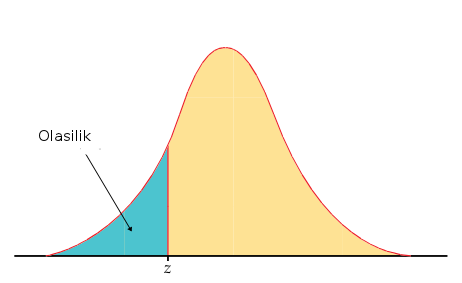
\includegraphics[height=4cm]{90_1.png}

\ \ z \ \ \  .00  \ \ \ .01 \ \ \ .02 \ \ \ .03 \ \ \ .04 \ \ \ .05 \ \ \ .06 \
\ \ .07 \ \ \ .08 \ \ \ .09

-3.4 .0003 .0003 .0003 .0003 .0003 .0003 .0003 .0003 .0003 .0002

-3.3 .0005 .0005 .0005 .0004 .0004 .0004 .0004 .0004 .0004 .0003

-3.2 .0007 .0007 .0006 .0006 .0006 .0006 .0006 .0005 .0005 .0005

-3.1 .0010 .0009 .0009 .0009 .0008 .0008 .0008 .0008 .0007 .0007

-3.0 .0013 .0013 .0013 .0012 .0012 .0011 .0011 .0011 .0010 .0010

-2.9 .0019 .0018 .0018 .0017 .0016 .0016 .0015 .0015 .0014 .0014

-2.8 .0026 .0025 .0024 .0023 .0023 .0022 .0021 .0021 .0020 .0019

-2.7 .0035 .0034 .0033 .0032 .0031 .0030 .0029 .0028 .0027 .0026

-2.6 .0047 .0045 .0044 .0043 .0041 .0040 .0039 .0038 .0037 .0036

-2.5 .0062 .0060 .0059 .0057 .0055 .0054 .0052 .0051 .0049 .0048

-2.4 .0082 .0080 .0078 .0075 .0073 .0071 .0069 .0068 .0066 .0064

-2.3 .0107 .0104 .0102 .0099 .0096 .0094 .0091 .0089 .0087 .0084

-2.2 .0139 .0136 .0132 .0129 .0125 .0122 .0119 .0116 .0113 .0110

-2.1 .0179 .0174 .0170 .0166 .0162 .0158 .0154 .0150 .0146 .0143

-2.0 .0228 .0222 .0217 .0212 .0207 .0202 .0197 .0192 .0188 .0183

-1.9 .0287 .0281 .0274 .0268 .0262 .0256 .0250 .0244 .0239 .0233

-1.8 .0359 .0351 .0344 .0336 .0329 .0322 .0314 .0307 .0301 .0294

-1.7 .0446 .0436 .0427 .0418 .0409 .0401 .0392 .0384 .0375 .0367

-1.6 .0548 .0537 .0526 .0516 .0505 .0495 .0485 .0475 .0465 .0455

-1.5 .0668 .0655 .0643 .0630 .0618 .0606 .0594 .0582 .0571 .0559

-1.4 .0808 .0793 .0778 .0764 .0749 .0735 .0721 .0708 .0694 .0681

-1.3 .0968 .0951 .0934 .0918 .0901 .0885 .0869 .0853 .0838 .0823

-1.2 .1151 .1131 .1112 .1093 .1075 .1056 .1038 .1020 .1003 .0985

-1.1 .1357 .1335 .1314 .1292 .1271 .1251 .1230 .1210 .1190 .1170

-1.0 .1587 .1562 .1539 .1515 .1492 .1469 .1446 .1423 .1401 .1379

-0.9 .1841 .1814 .1788 .1762 .1736 .1711 .1685 .1660 .1635 .1611

-0.8 .2119 .2090 .2061 .2033 .2005 .1977 .1949 .1922 .1894 .1867

-0.7 .2420 .2389 .2358 .2327 .2296 .2266 .2236 .2206 .2177 .2148

-0.6 .2743 .2709 .2676 .2643 .2611 .2578 .2546 .2514 .2483 .2451

-0.5 .3085 .3050 .3015 .2981 .2946 .2912 .2877 .2843 .2810 .2776

-0.4 .3446 .3409 .3372 .3336 .3300 .3264 .3228 .3192 .3156 .3121

-0.3 .3821 .3783 .3745 .3707 .3669 .3632 .3594 .3557 .3520 .3483

-0.2 .4207 .4168 .4129 .4090 .4052 .4013 .3974 .3936 .3897 .3859

-0.1 .4602 .4562 .4522 .4483 .4443 .4404 .4364 .4325 .4286 .4247

0.0 .5000 .4960 .4920 .4880 .4840 .4801 .4761 .4721 .4681 .4641

\newpage

\ \ z \ \ \  .00  \ \ \ .01 \ \ \ .02 \ \ \ .03 \ \ \ .04 \ \ \ .05 \ \ \ .06 \
\ \ .07 \ \ \ .08 \ \ \ .09

0.0 .5000 .5040 .5080 .5120 .5160 .5199 .5239 .5279 .5319 .5359

0.1 .5398 .5438 .5478 .5517 .5557 .5596 .5636 .5675 .5714 .5753

0.2 .5793 .5832 .5871 .5910 .5948 .5987 .6026 .6064 .6103 .6141

0.3 .6179 .6217 .6255 .6293 .6331 .6368 .6406 .6443 .6480 .6517

0.4 .6554 .6591 .6628 .6664 .6700 .6736 .6772 .6808 .6844 .6879

0.5 .6915 .6950 .6985 .7019 .7054 .7088 .7123 .7157 .7190 .7224

0.6 .7257 .7291 .7324 .7357 .7389 .7422 .7454 .7486 .7517 .7549

0.7 .7580 .7611 .7642 .7673 .7704 .7734 .7764 .7794 .7823 .7852

0.8 .7881 .7910 .7939 .7967 .7995 .8023 .8051 .8078 .8106 .8133

0.9 .8159 .8186 .8212 .8238 .8264 .8289 .8315 .8340 .8365 .8389

1.0 .8413 .8438 .8461 .8485 .8508 .8531 .8554 .8577 .8599 .8621

1.1 .8643 .8665 .8686 .8708 .8729 .8749 .8770 .8790 .8810 .8830

1.2 .8849 .8869 .8888 .8907 .8925 .8944 .8962 .8980 .8997 .9015

1.3 .9032 .9049 .9066 .9082 .9099 .9115 .9131 .9147 .9162 .9177

1.4 .9192 .9207 .9222 .9236 .9251 .9265 .9279 .9292 .9306 .9319

1.5 .9332 .9345 .9357 .9370 .9382 .9394 .9406 .9418 .9429 .9441

1.6 .9452 .9463 .9474 .9484 .9495 .9505 .9515 .9525 .9535 .9545

1.7 .9554 .9564 .9573 .9582 .9591 .9599 .9608 .9616 .9625 .9633

1.8 .9641 .9649 .9656 .9664 .9671 .9678 .9686 .9693 .9699 .9706

1.9 .9713 .9719 .9726 .9732 .9738 .9744 .9750 .9756 .9761 .9767

2.0 .9772 .9778 .9783 .9788 .9793 .9798 .9803 .9808 .9812 .9817

2.1 .9821 .9826 .9830 .9834 .9838 .9842 .9846 .9850 .9854 .9857

2.2 .9861 .9864 .9868 .9871 .9875 .9878 .9881 .9884 .9887 .9890

2.3 .9893 .9896 .9898 .9901 .9904 .9906 .9909 .9911 .9913 .9916

2.4 .9918 .9920 .9922 .9925 .9927 .9929 .9931 .9932 .9934 .9936

2.5 .9938 .9940 .9941 .9943 .9945 .9946 .9948 .9949 .9951 .9952

2.6 .9953 .9955 .9956 .9957 .9959 .9960 .9961 .9962 .9963 .9964

2.7 .9965 .9966 .9967 .9968 .9969 .9970 .9971 .9972 .9973 .9974

2.8 .9974 .9975 .9976 .9977 .9977 .9978 .9979 .9979 .9980 .9981

2.9 .9981 .9982 .9982 .9983 .9984 .9984 .9985 .9985 .9986 .9986

3.0 .9987 .9987 .9987 .9988 .9988 .9989 .9989 .9989 .9990 .9990

3.1 .9990 .9991 .9991 .9991 .9992 .9992 .9992 .9992 .9993 .9993

3.2 .9993 .9993 .9994 .9994 .9994 .9994 .9994 .9995 .9995 .9995

3.3 .9995 .9995 .9995 .9996 .9996 .9996 .9996 .9996 .9996 .9997

3.4 .9997 .9997 .9997 .9997 .9997 .9997 .9997 .9997 .9997 .9998




\end{document}



